\documentclass[tikz, border=1mm]{standalone}
\usepackage{tikz} 
\usetikzlibrary{arrows.meta}
\usepackage{pgfplots}

\begin{document}

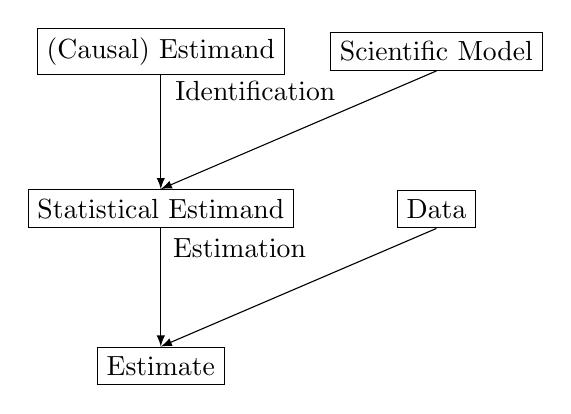
\begin{tikzpicture}
    % nodes
    \node at (0,2) [rectangle,draw]  {(Causal) Estimand};
    \node at (3.5,2) [rectangle,draw] {Scientific Model};
    \node at (0,0) [rectangle,draw] {Statistical Estimand};
    \node at (3.5,0) [rectangle,draw] {Data};
    \node at (0,-2) [rectangle,draw] {Estimate};
    \node at (1.2,1.5) {Identification};
    \node at (1,-0.5) {Estimation};
        
	% paths
    \draw[-{latex}](0,1.7) to (0,0.25); % CE -> SE
    \draw[-{latex}](3.5,1.75) to (0,0.25); % SM -> SE
    \draw[-{latex}](0,-0.25) to (0,-1.75); % SE -> E
    \draw[-{latex}](3.5,-0.25) to (0,-1.75); % D -> E
    
\end{tikzpicture}

\end{document}
